\section{Problem setup}
\label{sec:setup}
We use two domains as examples of general dynamic manipulation tasks, one featuring 1-D deformable objects (ropes) and the other focusing on 2-D deformable objects (table cloths). For both tasks, the physical parameters of the objects are not known to the algorithm a priori.
% During testing, a single policy is used for each task with different manipulands, robot embodiment, etc, demonstrating the method's generalization capability. 
During testing, a single policy is used for each task and evaluated across a diverse set of manipulands and robot embodiments, demonstrating our method's strong generalization capability to objects significantly outside of its training distribution.

\textbf{Rope whipping.}
The task is to hit a target location in the air with the tip of a rope attached to a UR5 robot (Fig \ref{fig:teaser} first row). The range of target locations far exceed the robot's reach range, requiring the robot to swing the rope dynamically. To reach sufficient speed in practice, we extended the UR5's end-effector with a 50cm long wooden stick. We use a parametric action primitive to describe the robot's movement. The action space for the whipping primitive is $a = (v, J_2, J_3)$, where $J_2 \in [90,-30]^{\circ}$ and $J_3 \in [-110,-290]^{\circ}$ are the target angles for joints two and three, respectively, and $v \in [1.0,3.14]$ \si{rad/s} is the maximum permissible angular velocity across all joints. 



This action primitive considers only 2D movement in the Y-Z plane, where target locations are defined in-plane --- it is sufficient for this task, since out-of-plane goals could be reached simply by rotating the robot's base joint. 
The trajectory of the rope tip $T_i$ is tracked and rasterized to a $256^2$ image as observation input.
The distance metric $\mathcal{D}(T_i,g)$ for this task is defined as the minimum distance from any point on the trajectory $T_i$ to the goal location $g$.

%modeled after the UR5 robot's movej command: joint 2 and 3's angular goal as well as maximum angular velocity.  
%The actual robot movement is implemented as linear movement in joint space from a fixed initial joint configuration. The movement follows a trapezoidal speed profile with a constant acceleration of $10$ \si{rad/s^2}. 
%The robot moves linearly in joint space, following a trapezoidal speed profile with a constant acceleration of $10$ \si{rad/s^2}. We have set upper and lower limits for each dimensions of the action space to prevent self-collision.
%We assume that the robot only moves in a 2D plane and only consider in-plane goals. We believe this action space is sufficient for this task, since out-of-plane goals can be reached by rotating the robot's base joint. 

\textbf{Cloth placement.}
The task is to place a square cloth on the table that reaches the goal configuration specified by 9 keypoints on the cloth (shown in Fig. \ref{fig:teaser} bottom row). Again, the goal configurations are further than the arm's maximum reach range, requiring dynamic actions. We assume that the cloth is gripped by two grippers that move in sync and consider the case where the grippers only move within the Y-Z plane, since out-of-plane goals can be reached by horizontally translating the trajectory. Gripper trajectory is parameterized as a cubic spline with $3$ via-points, evenly spaced temporally, in the Y-Z plane, Fig. \ref{fig:cloth_plot}. The start point and the Z coordinate for the end point are fixed. The remaining 3 degrees of freedom --- Y,Z locations for the second via-point and the Y locations of the third via-point--- as well as the total duration of the action, constitute the $4$ dimensional action space. The trajectory for all $9$ keypoints on the cloth $T_i$ is used as input observation to the algorithm. 
The distance metric $\mathcal{D}(T_i,g)$ for this task is defined as the mean keypoint distance between the cloth's final configuration and target configuration. 

\section{Approach}

\begin{figure}
    \centering
    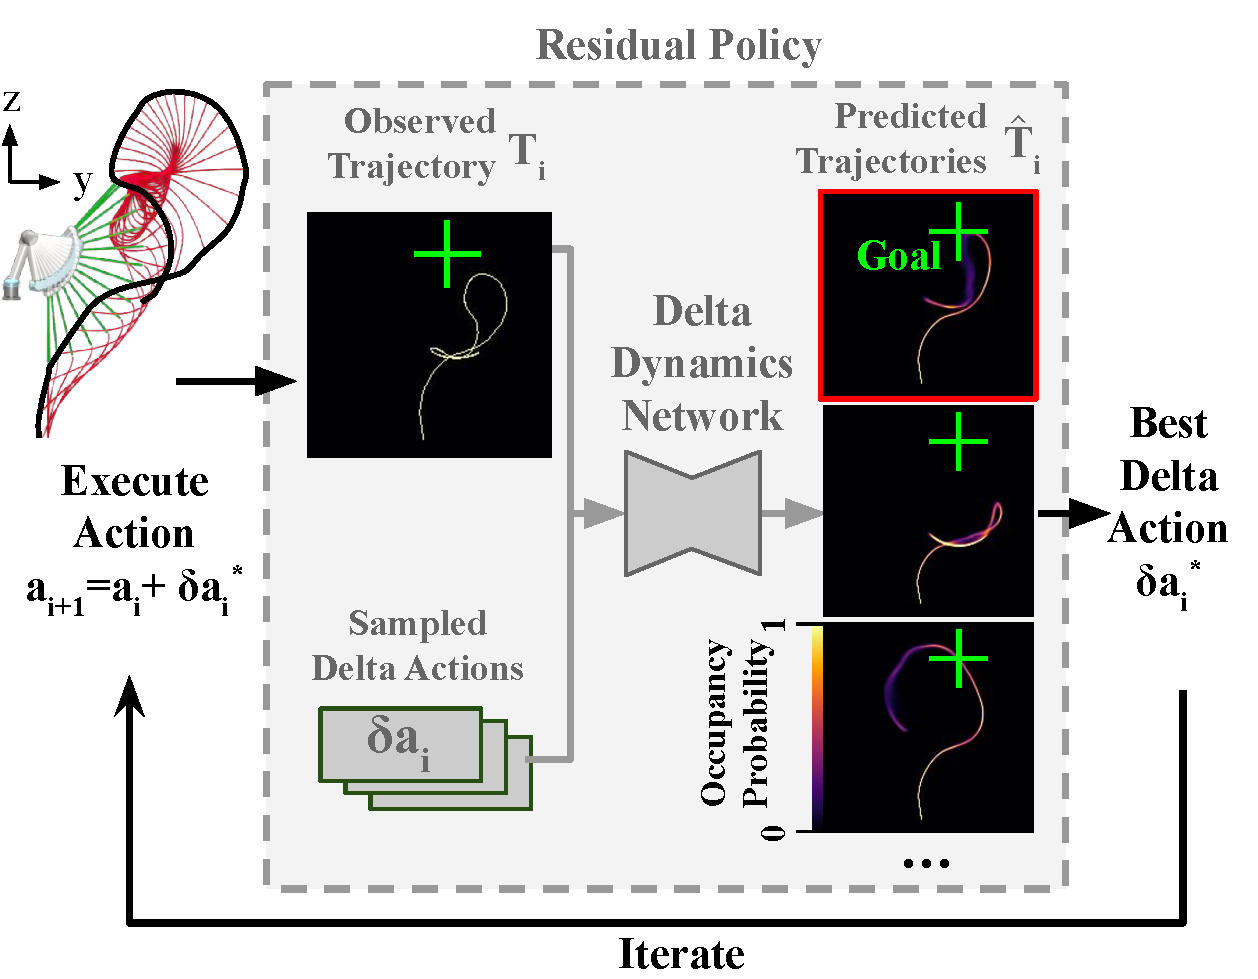
\includegraphics[width=\linewidth]{figure/rope-pipeline.pdf}
    \caption{\textbf{\namel}. During each action execution, the tip trajectory is recorded as an image. For each sampled delta action $\delta a$, the Delta Dynamics Network predicts trajectories resulting from applying each delta action. The delta action that is predicted to minimize distance to the target is selected for execution during the next iteration.}
    \label{fig:method} \vspace{-1mm}
    % https://docs.google.com/drawings/d/1mfCcU8B-Oooa7aT68fllYr_3jWxToHtNDBJuhM9C9ZA/edit
\end{figure}

\begin{algorithm}[t]
\caption{Iterative Residual Policy} \label{alg:IRP}
\begin{algorithmic}[1] 
\STATE Input: Goal position $g$
\STATE Initialize action $a_0 \in \mathbb{R}^{N_a}$ \hspace{0.1in} $\triangleright$ \S\ref{sec:method_sample} Initial action
\WHILE{$i <$ max\_step}
    \STATE $T_i$ = robot\_execution($a_i$) 
    \STATE $d_i$ = $\mathcal{D}$($T_i$, $g$) \hspace{0.5in} $\triangleright$ \S\ref{sec:setup} Defined for each task
    \IF{$d_i < d_{stop}$ }
        \STATE break;
    \ENDIF
    \STATE ${\delta a_i^{0:N_s}}$ = sample\_action($d_i$)  \hspace{0.2in} $\triangleright$ \S\ref{sec:method_sample} Delta action
    \STATE ${\hat{T}_i^{0:N_s}}$ = delta\_dynamics($\delta a_i^{0:N_s}$, $T_i$)   {\hspace{0.2in} $\triangleright$ \S\ref{sec:method_RDM}}
    \STATE $j^* = \argmin_{j}$($\mathcal{D}$($\hat{T}_i^{j}$,$g$))
    \STATE $a_{i+1}$ = $a_{i} + \delta a_i^{j^*}$
\ENDWHILE
\end{algorithmic}
\end{algorithm}

When attempting to hit a target with an unfamiliar rope, humans will generally not succeed on their first try. However, using physical intuition, people can usually \textbf{predict the effect of adjusting their actions}; when swinging a rope, for example, larger force will make the rope tip swing higher. Although the prediction is not perfect, people often adjust their actions in the right direction and quickly drive down their error after a few interactions.

Building on this intuition, we propose \textbf{Iterative Residual Policy} for goal-conditioned dynamic manipulation of deformable objects. Given an observation of trajectory $T_i$ by action $a_i$, we sample a set of potential delta actions $\delta a_i$ and predict the resulting trajectory $\hat{T}_i$ for each delta action. We then evaluate each of the predicted trajectories based on their minimal distance to the goal $d_i$, and greedily select the optimal delta action $\delta a_i^{j*}$ to execute in the next iteration. Trained using simulation data alone, this method is able to achieve high accuracy and generalize to out-of-distribution objects on our real-world robot setup. The following sections provide details for the key algorithm components and design decisions. 

\begin{figure*}[t]
    %\centering
    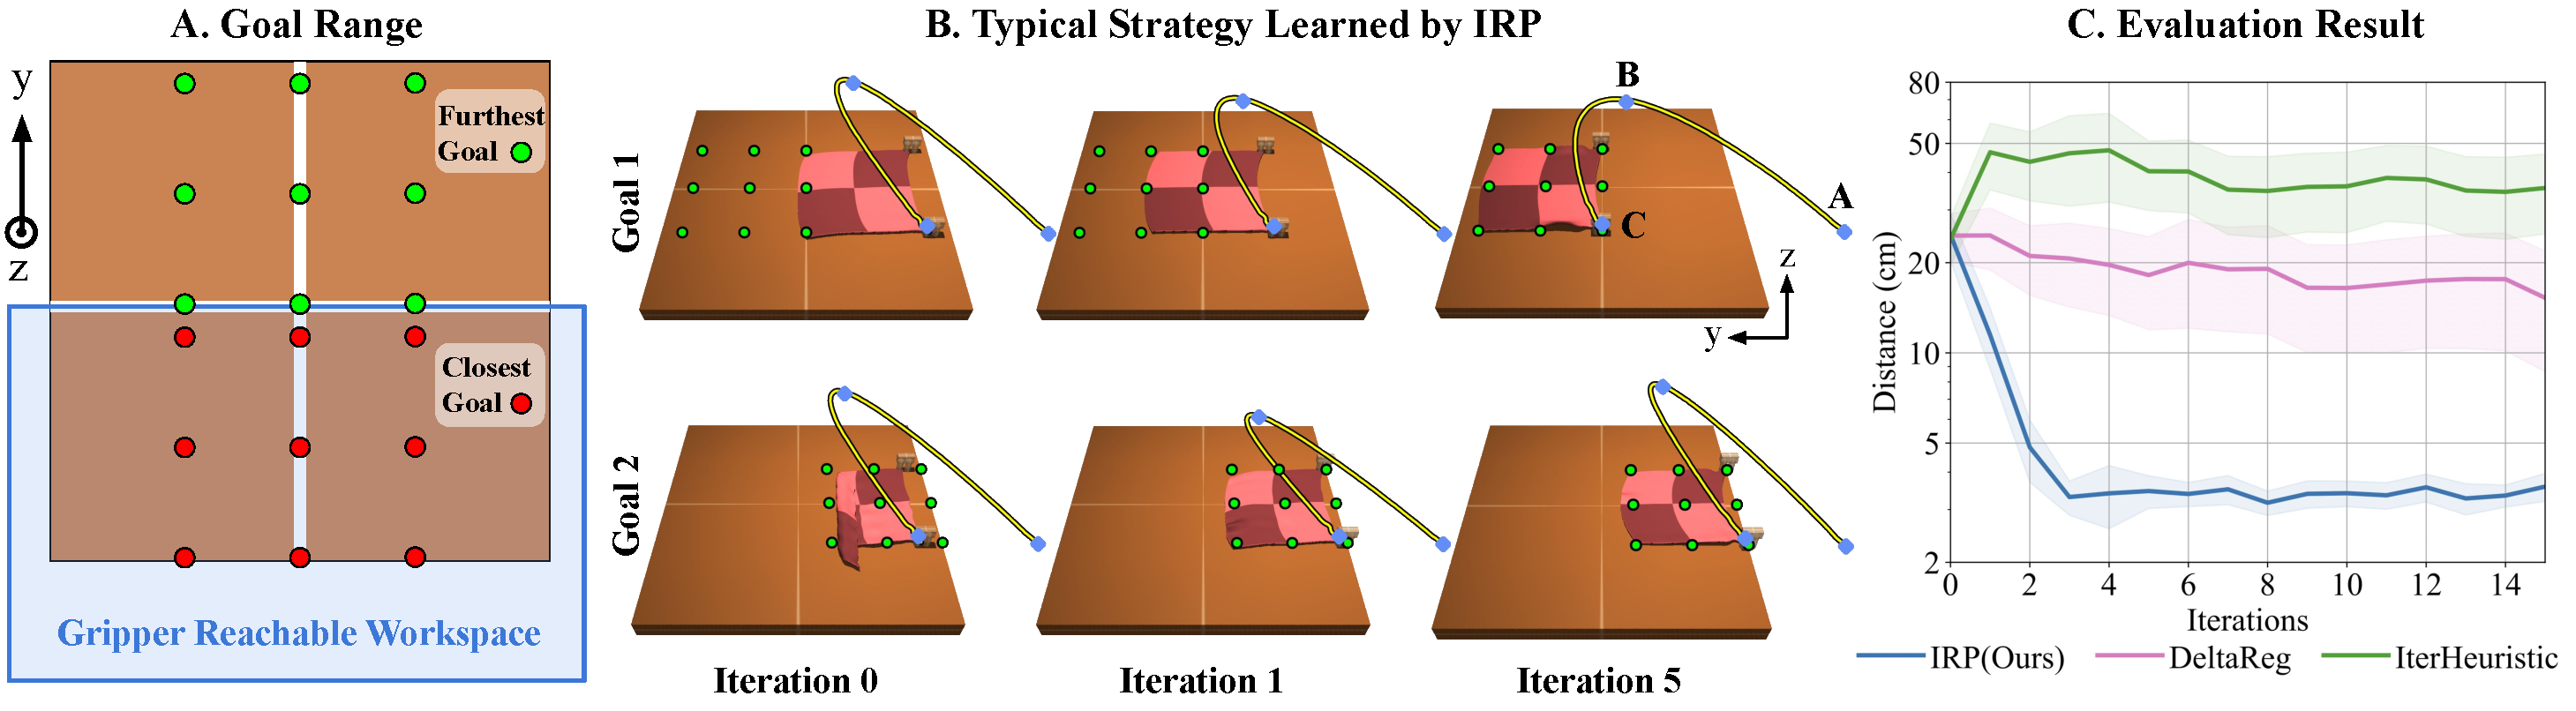
\includegraphics[width=\linewidth]{figure/cloth_plot.pdf}
    \caption{\textbf{Cloth placing task} A) Some goals are placed outside the arm's reach range, therefore requiring dynamic actions. 
    B) Top row: our algorithm adjusts the trajectory to reach a far-away goal. Bottom row: our algorithm reduces action velocity to eliminate undesired folding.
    C) Mean distance to goal keypoints averages across all test cloth and goals, shown with a 95\% confidence interval. Our method yields significantly better performance compared to the [deltaReg] baseline. Note that due to the stretching of the cloth and thickness of collision capsules, it is not possible to achieve 0 error. }
    \label{fig:cloth_plot} \vspace{-4mm}
    % https://docs.google.com/drawings/d/1qIPaECj8m26UyuAT7611URPWJPjAzNO1Q7S1zr13SZE/edit?usp=sharing
\end{figure*}




\subsection{Delta Dynamics Network}
\label{sec:method_RDM}
The delta dynamics network takes in an observed trajectory $T_i$ and a delta action $\delta a_i^j$ as input and predicts the trajectory ${\hat{T}_i^{j}}$ after the delta action is applied. This network is used at every iteration for action optimization. 


\textbf{Trajectory representation.}
To spatially represent the trajectory $T_i$, we rasterize the it into a $256\times256$ image projected onto the Y-Z plane. $T_i$ covers $\pm 3m$ area from the robot base joint. 
The pixel values correspond to occupancy probability; the observed trajectories have a binary pixel and the predicted trajectories are real-valued: $p \in [0,1]$. For the cloth placing task, the trajectory image of all 9 keypoints are stacked channel-wise.
Due to small differences in initial condition, hardware precision, ambient airflow as well as other disturbances, the trajectory is not always the same for each action. Moreover, different segments of the trajectory exhibit different sensitivity to noise. 
% We observed that by including trajectory uncertainty in the training data in the form of initial state perturbations, the model learns to prefer regions of space with higher repeatability.
 

\textbf{Action representation.}
We broadcast the $N_a$ dimensional delta action $\delta a_i$ into a $N_a$ channel image and then concatenate them with the trajectory images before feeding them into the network. This spatially aligned representation allows us to use a standard CNN  architecture designed for image segmentation while ensuring the action information is available in the receptive field of every neuron.
% \shuran{what is visible from every part of the network mean? I understand, but I don't think reader will. }


\textbf{Network and loss.}
We use DeepLabV3+ \cite{deeplabv3} for our network architecture. During training, we uniformly select actions as $a_i$ and sample $\delta a_i$ with a Gaussian distribution (SD=0.125). The resulting trajectories in simulation are used as supervision. The network is trained with Binary Cross Entropy Loss and the AdamW optimizer \cite{adamw} with learning rate of 0.001 and weight decay of $1\times 10^{-6}$.
% \shuran{how you get the supervision for your output? what loss you use to train the network?} 
% \shuran{learning rate or other details}


\subsection{Interactive Action Sampling and Selection}
\label{sec:method_sample}
\textbf{Initial action.} In the rope whipping task, the initial action $a_0$ is selected using the best average action for all training rope given a specific goal. This action can be computed efficiently with our offline training dataset.
The same action is used for a goal regardless of the rope parameters.
In the cloth placement task, a constant initial action is used for all goals to ensure all keypoint trajectories are observable in the first iteration. 


\textbf{Delta action.}
Since each dimension of the action space has been scaled to between 0 and 1, we sample $N_s=128$ delta actions $\delta a_i$ for each iteration from a spherical Gaussian distribution with 0 mean and standard deviation $\sigma$. To reduce overshooting and accelerate convergence, we select $\sigma = 0.5 \times d_i$, where $d_i =\mathcal{D}(T_i,g)$.


\textbf{Action selection.}
After the network predicts the raw trajectories image for all delta action sample $\delta a_i^{0:N}$, we threshold the prediction with $t=0.2$, creating a set of binary trajectory image $\hat{T}_i^{0:N}$. 
Then, the delta action $\delta a_i^{j*}$ associated with smallest distance $\mathcal{D}(\hat{T}_i^{j},g)$ is selected to compute next action: $a_{i+1} = a_i + \delta a_i^j$. 
In real-world experiments, the optimization stops when the policy reaches $\mathrm{d\_stop}=2cm$ error or maximum iteration $\mathrm{max\_step}=10$ is reached. In simulation, the optimization executes for exactly $16$ iterations. The algorithm is summarized as pseudocode in Algorithm \ref{alg:IRP}.

\begin{figure*}[t]
    \centering
    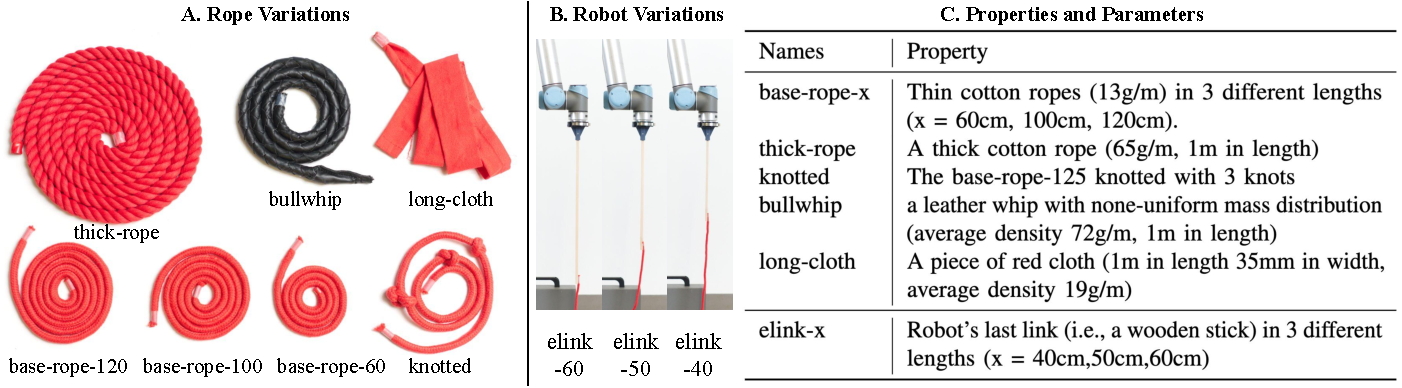
\includegraphics[width=\linewidth]{figure/Rope-realtest.pdf}
    \caption{ \label{fig:testcase} \textbf{Real-world test cases.} A) Real-world testing ropes used to test our algorithm's generalization to untrained material, length, mass distribution and aerodynamics. B) By changing the the length of last link, the mapping from action parameters to effective swing speed and end-effector trajectory are changed simultaneously.  C) Table for key properties and parameters for each real world test case.}   
    %https://docs.google.com/drawings/d/1NQgDbs0Qv8fhNQQ7Cnk_LRvdaXN0g8vT9eRwg_KY090/edit?usp=sharing 
    \vspace{-3mm}
\end{figure*}

\subsection{Training Data Generation}
\label{sec:data_generation}

\textbf{Rope whipping.}
For training and validation, we built a simulation environment in MuJoCo \cite{mujoco}. The rope is simulated using 25 linked capsules and to generate different ropes, varying two parameters: length and density. The range of both parameters as well as the training/testing split is shown in Fig. \ref{fig:sim} left.  
The rope parameters are sampled from a $12^2$ grid. For each rope, we simulate $50^3$ actions within the set box constraint for speed $[1,3.14]$ \si{ rad/s}, joint 2 $ \in [90, -30]^{\circ}$ and joint 3 $\in [-110, -290]^{\circ}$. In addition, each action was repeated 3 times with different random perturbations on the initial state to capture the stochastic nature of the trajectory. The entire dataset contains 54 million trajectories.

Clearly this model does not capture all the variations in real-world ropes, and the simulation itself presents different dynamics from the real world due to unmodeled factors such as aerodynamics, collision with the floor, etc. Despite the significant sim-to-real gap, we will later show that our model trained on these simulated ropes generalizes very well in the real world with significantly out-of-distribution ropes. %\cheng{due to our iterative online adaption formulation. In contrast, algorithms that produces the optimal action in training directly does not transfer well to realworld experiments.}

\textbf{Cloth placement.}
Similarly, the training data for cloth is collected from a MuJoCo simulation environment. The square cloth is simulated as a $13^2$ grid of capsules, skinned as a cloth for visualization. We again vary 2 parameters: size (ranged between 0.4 to 0.6 m) and density (ranged between 0.2 to 1.4 \si{kg/m^2}). For each cloth parameter, we sample speed and 3 via-point parameters from a $8\times16^3$ grid. In total, the dataset contains 131 thousand examples.

\subsection{Real world system setup.}
We conducted real-world experiments for the rope whipping task with an UR5-CB3 robot augmented with a wooden extension. We used a single RGB camera (Stereolab ZED 2i) running at 720p 60fps for tracking the tip of the rope. Due to the limited resolution and large motion range, stereo tracking does not provide sufficient depth accuracy and reliability. We therefore assume that the rope tip only moves in a 2D plane, allowing us to reduce the perception problem to that of 2D tracking. We placed the camera 2.4m away from the robot, and calibrated the homography between the image plane and the robot Y-Z plane with manually labeled point correspondences. We trained a keypoint detection model based on DeepLabV3+ with 400 hand labeled images.
Note that we use a higher image resolution (720p instead of 256p) for tracking results with less than 1.3cm tracking error in the validation set.

\begin{figure*}[t]
    \centering
    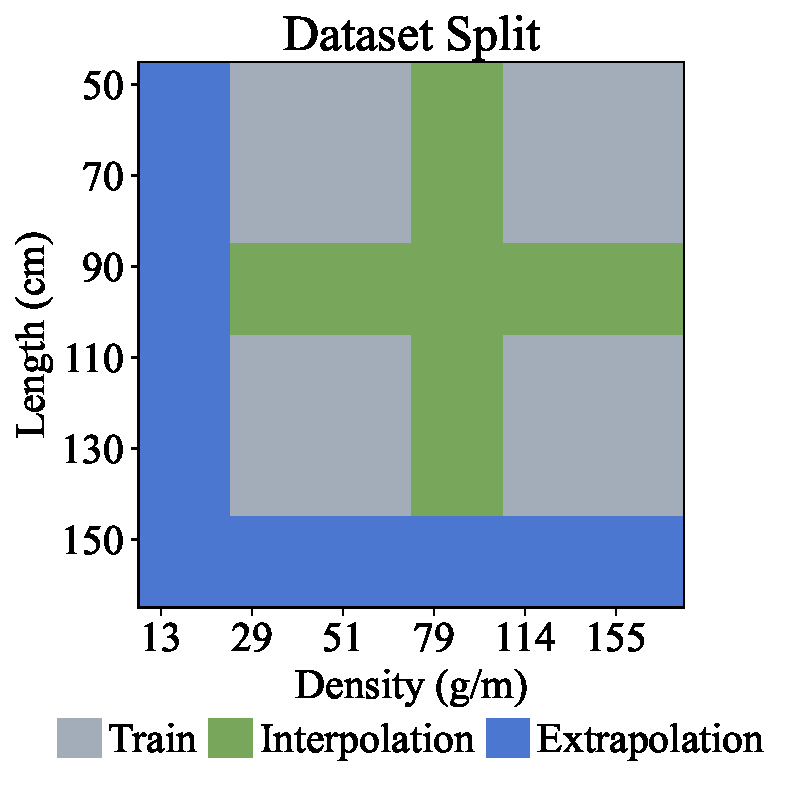
\includegraphics[width=0.264\linewidth]{figure/split_plot.pdf}
    \hspace{-4mm}
    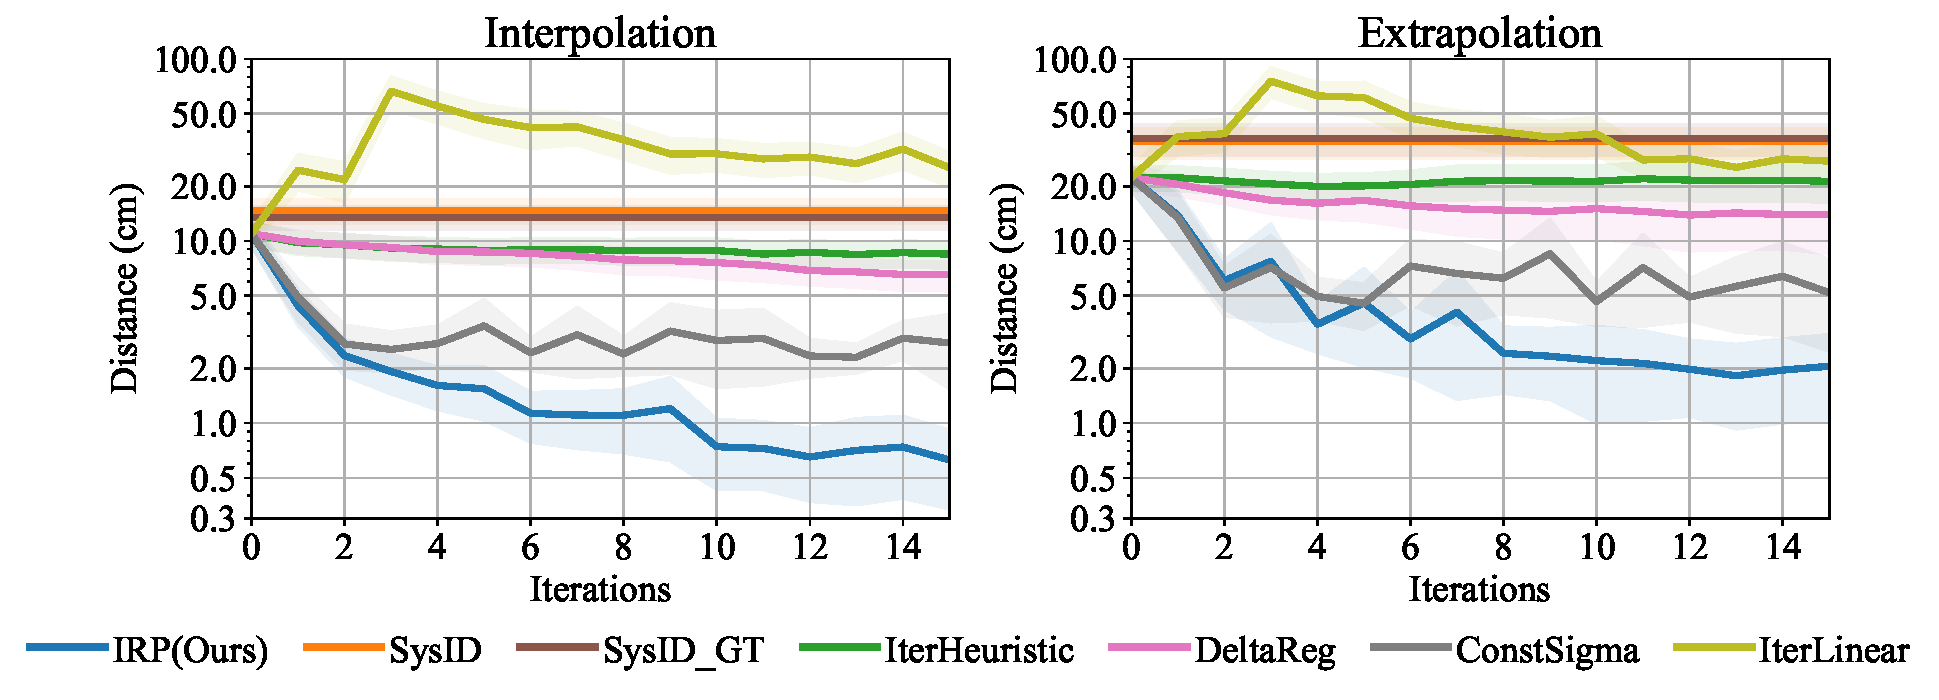
\includegraphics[width=0.736\linewidth]{figure/sim_plots.pdf}
    \vspace{-1mm}
    \caption{\textbf{Rope Experiments in Simulation.} Left: $12\times12$ grid of rope parameters used in simulation experiment (grey: training, orange: interpolation, blue: extrapolation). Middle and Right:  Distance to goal in cm averaged across 5 ropes and 25 goals for each method, shown with 95\% confidence interval. The result of single-step methods (SySID, SySID\_GT) are shown as lines for visualization.
    Testing rope with parameters that extrapolate  beyond training ropes parameters (middle) typically result in higher distance errors for most of the alternative approaches. However, \names is able to achieve low distance errors for both scenarios (0.4cm and 1.5cm respectively).} 
    \vspace{-3mm} 
    \label{fig:sim}
\end{figure*}